% !TeX root = ../dissertation.tex
\section{Methodology}
\label{sec_method}

All experiments were run on a Dell Precision 3620 workstation with NVIDIA
Quadro~6000 GPU and Intel Xeon CPU E5-2643 (3.40GHz) CPU. We implemented or ported all prototypes
and benchmarks on Ubuntu~16.04 with Xen~4.8.2. VMs were hardware-accelerated via Xen Hardware
Virtual Machines (HVM) with 2~virtual CPUs (pinned) and 4~GB memory.
% \aak{Kernel version...}

Of the GPU hardware available to us, the NVIDIA Quadro~6000 GPU was the only one that GPUvm, the
full-virtual\-ization baseline ran on. GPUvm depends on GDev~\cite{gdev}
 % make it impossible to run GPUvm on newer GPUs. GDev is
an open source CUDA runtime (released in 2012) implemented using Nouveau~\cite{nouveau} GPU
drivers, and the CUDA~4.2 compiler on Linux Kernel~3.6.5. GDev has not been maintained since 2014,
and the effort to update it was too onerous.
% This restricted all of our evaluation to the Quadro 6000.
Experiments to control for hardware versions are reported in \ref{sec:control}.
% GPUvm relies heavily on reverse-engineered details of a small set of NVIDIA GPUs.
% Of the GPUs available to us, the NVIDIA Quadro 6000 was the only one that was compatible.
% experiments to control for the datedness
% of the Quadro 6000 (presented in section~\ref{sec:control}) indicate that our findings hold for
% more current hardware.

\subsection{Benchmarks}
% \trxd and \trxc depend on the Mesa3D using the Clover OpenCL runtime.least
\trxc depends on the TGSI back-end compiler that we implemented to leverage
the Clover OpenCL runtime in Mesa3D.
% The compiler back-end can produce correct
% TGSI output for 10 of the Rodinia benchmarks at the time of submission, all of
% which we could execute on \trxc.
\apigpu and \apicpu leverage the NVIDIA and Intel OpenCL library respectively
and support all of the Rodinia benchmarks.
GPUvm is built on top of the GDev CUDA runtime.
% , and can correctly execute at least the same 10 benchmarks that run on \trxc.
Care was taken to ensure that the CUDA and OpenCL versions of the benchmarks use the same
parameters, datasets, memory barriers, sync points, etc. Experiments to
control for the programming framework are reported in \ref{sec:control}.


\newcommand{\RowColor}{\rowcolor{red!50} \cellcolor{white}}
\newcommand{\NewBncColor}{\cellcolor{green!25}}
\newcommand{\FailBncColor}{\cellcolor{gray!50}}

\begin{table}[!ht]
  \centering
  \caption{\small\uppercase{Evaluation Benchmarks in three categrories}$^{\mathrm{a}}$}
  \small
  \begin{tabular}{|r|l|c|}
    \hline
    \textbf{Benchmark} & \textbf{Description} & \textbf{Type} \\ \hline
    backprop & Back propagation (pattern recognition) & R \\ \hline
    % bfs & Breadth-First Search \\ \hline
    gaussian & 256x256 matrix Gaussian elimination & D \\ \hline
    % hotspot & Hotspot (physics simulation) \\ \hline
    lud & 256x256 matrix LU decomposition & M \\ \hline
    nn & $k$-nearest neighbors classification & D \\ \hline
    nw & Needleman-Wunsh (DNA-seq alignment) & M \\ \hline
    pathfinder & Search shortest paths through 2-D maps & R \\ \hline

    \multicolumn{3}{l}{\footnotesize{$\mathrm{a}.$ Interposition-$\mathbf{d}$ominant, interposition-$\mathbf{r}$are, and $\mathbf{m}$oderate workloads.}}
  \end{tabular}
  % \hyu{Table out of place}
  \label{tb_bench}
  % \label{tb_fail_bench}
\end{table}

%Due to the space limitation \hyu{modify reminder},
% \hyu{Our under-development TGSI compiler supports xxx instructions, and is able to compile 10 ...}
The 10 Rodinia benchmarks that our TGSI compiler could compile were categorized based
on frequency of interposition:
Interposition-\textbf{D}ominant workloads run kernels hundreds or thousands of times requiring
frequent interposition to set arguments, etc.
Interposition-\textbf{R}are workloads run a small number of long-running kernels, requiring very little interposition.
\textbf{M}oderate-interposition workloads lie somewhere in between the other two.
Two benchmarks were selected from each category
to be used in the evaluation
(the optimizations described in \ref{sec:optimizations} take significant manual effort).

% These benchmarks are shown in Table~\ref{tb_bench}.
% enabling overheads to be hidden by the speedup of \texttt{Init} time (pre-initialized by remote server).
%We fixed some minor bugs, added instrumentation code, and set the appropriate block size and number of \texttt{threads\_per\_block} for the test system.
%We modified the \texttt{nn} benchmark to run the GPU kernel multiple times because the GPU kernel execution time of the default benchmark was too short.

% For each benchmark, we report the time spent in the following phases ---
% initialization, data transfer, and kernel execution time (on the GPU), and
% close. The \texttt{close} phase, in which applications usually unload modules,
% free device memory and destroy context, is negligible for OpenCL benchmarks
% (as the OpenCL runtime performs these operations asynchronously), but is a
% source of significant slowdown in applications run on the GDev CUDA framework.
% applications (run on GPUvm).
% are non-trivial.

\subsection{Control Experiments}
\label{sec:control}

Software and platform version dependencies necessitated that our experimental environments vary slightly for the systems under evaluation ---
% Meaningful comparison of different GPU virtualization designs then becomes a challenge
different front-end programming languages (CUDA vs. OpenCL), different runtime
implementations (GDev CUDA vs. NVIDIA CUDA), or different drivers (Nouveau vs. NVIDIA).
Resolving all of these differences would have taken monumental effort, but control experiments showed that these variables had negligible impact on our measurements.

\paragraphbe{OpenCL vs. CUDA} GPUvm relies on the GDev implementation of the
CUDA framework, while all the other designs rely on OpenCL. To assess the
impact of different front-end languages on performance, we measured execution
times for all benchmarks in both CUDA and OpenCL (Rodinia includes both
implementations) holding all other variables constant, and found that the
front-end language has near negligible impact, and the harmonic mean of
differences in kernel execution time across all benchmarks is less than 1\%;
the worst (maximal) case is 15\%.
We also found negligible difference in performance between kernels compiled using CUDA 8.0 and the CUDA 4.2 required by GDev.

%We performed additional measurements
%to control for noise with CUDA compiler versions and found negligible
%error between kernels compiled with version 8 and the 4.2 version required
%by GDev.

%% \paragraphbe{CUDA runtime and compiler implementations}
%% The NVIDIA CUDA implementation is not open source, so experiments with system
%% software for CUDA are generally forced to use \texttt{gdev}, which as an open
%% source implementation, reverse-engineered and maintained by a handful of
%% researchers, has not enjoyed the optimization effort devoted the NVIDIA
%% production runtime.
%% Similarly, the NVIDIA \texttt{nvcc} compiler has evolved considerably between
%% the 4.2 version which \texttt{gdev} depends on and the most recent production
%% version at the time of this writing (\texttt{nvcc 8}). To control for noise
%% induced by these differences, we compare execution times using NVIDIA's
%% runtime with the version 8 and 4.2 compilers and \texttt{gdev} with the 4.2
%% compiler and Nouveau driver.


%% \begin{figure}[!ht]
%% 	\centering
%% 	\hspace*{-0.75cm}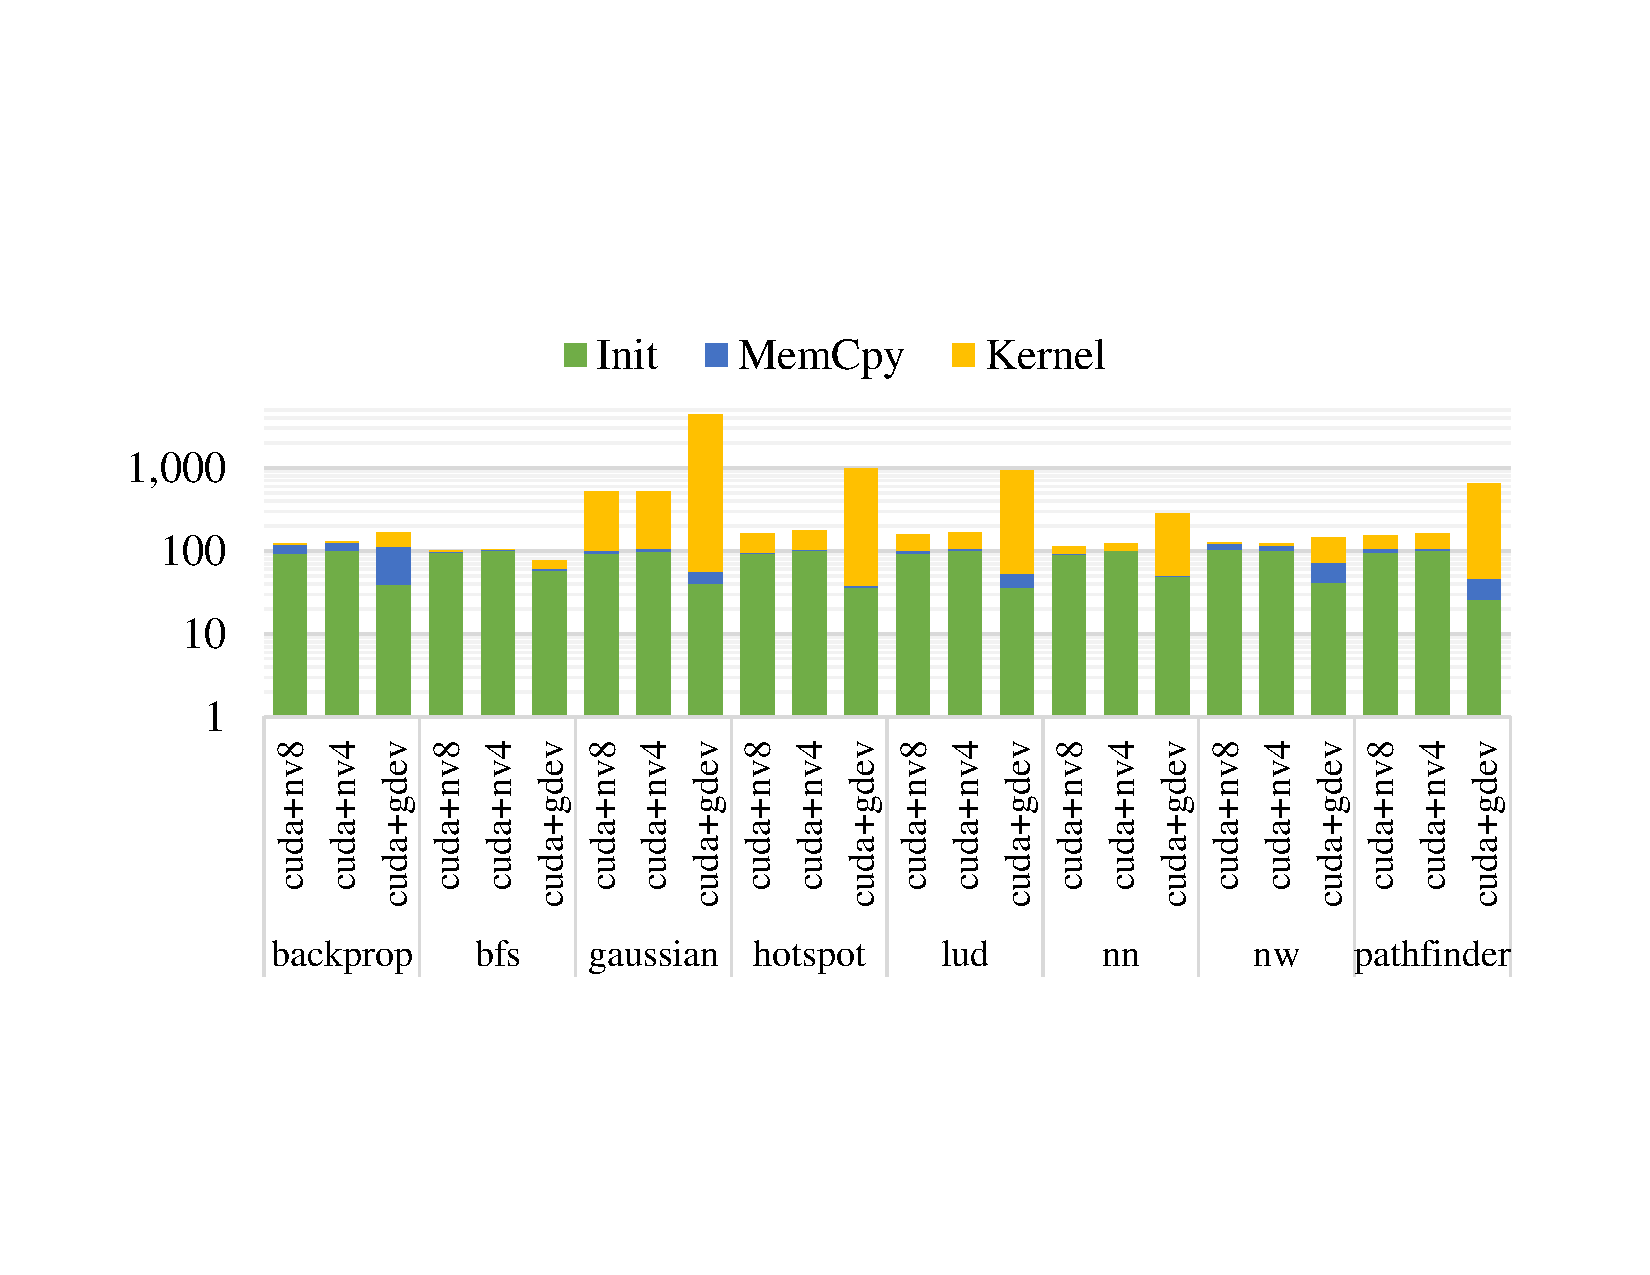
\includegraphics[width=1.1\linewidth,trim={2.3cm 5cm 2cm 5cm},clip]{data/basic/compiler.pdf}
%% 	\caption{{\footnotesize Runtime of benchmarks written in CUDA comparing impact of compiler version (NVCC 4.2 vs NVCC 8.0)
%% 		and runtime implementation (CUDA vs \texttt{gdev}).	Note that \texttt{gdev} depends on NVCC 4.2.}}
%% 	\label{fig_compiler} \end{figure}


%% Figure~\ref{fig_compiler} shows these results. When the NVIDIA stack is used,
%% the \texttt{nvcc} version has negligible impact, but there are important
%% differences introduced by \texttt{gdev}. While memory copy and kernel execution
%% times are often the same, \texttt{gdev} performs initialization more
%% quickly, but in some cases results in significantly longer kernel execution
%% times, e.g. \texttt{gaussian}, for which kernel time is over an order of
%% magnitude slower. To understand how runtime implementation can impact GPU side
%% execution time, recall that the front end CUDA compiler produces an IR (PTX)
%% which is finalized to the native ISA (SASS) by a JIT compiler \emph{in the
%% driver}. The PTX to SASS finalization in the NVIDIA Runtime is clearly better
%% optimized than the one used by \texttt{gdev} (implemented by the Nouveau
%% driver).

%% The harmonic mean delta between \texttt{gdev} and NVIDIA runtimes is X\%
%% and the distribution is bimodal. Consequently, controlling for variability
%% introduced by comparisons of designs that use it is difficult. Because
%% it remains an essentially open variable, we are careful to point out
%% scenarios in which it may introduce significant experimental noise.
%% \cjr{We need to sort this out. harmonic mean delta is around 1000\%
%% pretty consistently. Moving on while sorting this out with Hangchen.}
%% \hyu{Don't get the point of this paragraph.. If we don't normalize the runtime with
%% different baselines, why does this really matter?}

%The \texttt{Init} is faster in GDev because the runtime finishes part of the initialization work
%before application's main function starts.
%GDev has much more overheads than \cite{gdev}, probably because
%of the different settings of Xen and physical devices.
% \subsection{Compilation optimization}
% \label{sec_compilation}
% We use NVCC~4.2 to compile the CUDA kernel for GDev, while we use NVCC~8 in all other situations.
% To clarify the possible optimization brought by newer compiler and GPU driver, we compare the
% benchmarks' performance with CUDA toolkit 4.2 and 8.0.

\paragraphbe{Hardware Generations.} The performance improvements over the
span of generations between the Quadro 6000
%(on which most of the systems have a dependency)
and modern cards is substantial. To estimate the effect of this variable we
ran all benchmarks on both Quadro 6000 and a more recent GPU, Quadro P6000.
While overall execution times are improved substantially, and the ratio of
time spent on the host to time spent on the GPU changes as a result, the
relative speedups are uniform across all benchmarks. This suggests that the
trends that we observe on the Quadro 6000 still hold on newer hardware. We
re-iterate that software dependencies of the GPUvm baseline prevent us
from using more recent hardware. Our evaluation is performed on the newest
(several generations older) GPU hardware that all our systems can run on.
% but this finding suggests that our findings will continue to hold as
% virtualization systems catch up with current hardware generations.
% \cjr{Reasonable? I think we did something like this, didn't we? Or am
% I making it up?} \hyu{Reasonable. But shall we also mention the new GPU
% features that can improve the virtualization performance (e.g pagefault)?}
